\section{Targeted validation of heterogeneous semantic alignment}\label{sec:supp_deep}
\subsection{Anchored identification under a score margin}
Fix the provisional event groups and let $\mathcal E$ contain every nonconstant receiver-pair term in the map objective; constant terms cancel in objective differences. Assume the graph $(\{0,\ldots,S-1\},\mathcal E)$ is connected, receiver 0 has its true known map, every candidate map is a bijection, and any disclosed anchors agree with the true map. Write $R_{st}(\mathbf M)$ for the relative native-column permutation. An edge score depends on $\mathbf M$ only through this permutation.

For each edge, assume an ideal score $\psi^*_{st}$ has a unique maximum at $R^*_{st}$. Its minimum gap to a wrong relative map is $\delta_{st}>0$. The observed table is $\widehat\psi_{st}$. Assume
\[
 \sup_R\left|\widehat\psi_{st}(R)-\psi^*_{st}(R)\right|\leq\varepsilon_{st},
 \qquad \delta_{st}>2\varepsilon_{st}.
\]
For a feasible candidate $\mathbf M\ne\mathbf M^*$, let $D(\mathbf M)$ contain edges with a wrong relative map. This set is nonempty. Otherwise connectivity would propagate the true relative maps from the known reference to every source. The observed objective difference satisfies
\[
 \widehat J(\mathbf M^*)-\widehat J(\mathbf M)
 \geq\sum_{(s,t)\in D(\mathbf M)}
       (\delta_{st}-2\varepsilon_{st})>0.
\]
Unchanged relative maps contribute exactly zero to this difference, so the true anchored map is the unique optimum. This sufficient condition follows from the usual global naming freedom in permutation synchronization. It is stronger than necessary, since joint evidence may resolve cases with some ambiguous edges. The argument provides neither a recovery theorem for the RF generator nor an estimated sample-size threshold.

For a component without a known map or sufficient anchors, a common renaming preserves every internal relative map. For uniform posterior vectors, every relative permutation has the same compatibility. If two native columns are indistinguishable in all observations, swapping them also preserves the scores. When at least two admissible maps remain, these score symmetries prevent identification from the observations. Correct event groups alone cannot remove that ambiguity.

\subsection{Independent map comparison and computational checks}
The script is \texttt{code/deep\_mapping.py}. Replication indices are $r=0,\ldots,9$. Adaptation seeds are $100{,}000{,}000+100{,}000r+j$ for $j=0,\ldots,39$. Test seeds are $101{,}000{,}000+100{,}000r+j$ for $j=0,\ldots,79$. Hidden maps use seed $102{,}000{,}000+r$. Receiver 0 retains a known map. Receivers 1, 2, and 3 have no disclosed anchors. Their four-class maps remain fixed across adaptation and test. Budgets 1, 5, and 40 use adaptation prefixes. The comparison reports all budgets and all scorers. Test references select no parameters or map update.

The linear fits are read from the retained parameter files. The boosted model is reconstructed from the original 120 training scenes per replication. It uses the original hyperparameters and saved temperature. The script \texttt{code/deep\_scoring.py} compares every scorer with the retained 800-scene predictions. All 3200 scorer--scene partitions agree. Linear probabilities agree exactly. The largest boosted probability difference is $4.43\times10^{-11}$. This check concerns numerical reconstruction of frozen evidence.

All map estimators use the same initial physical-only groups. Reference-only fitting uses receiver-0 pair terms. Coordinate fitting starts from the identity completion. It allows up to 100 strict-improvement sweeps. Spectral fitting takes the best relative permutation for each observed receiver pair. Missing pair terms contribute zero blocks. Diagonal blocks are identity matrices. The symmetric block matrix supplies its top-$K$ eigenspace. Reference-block products are rounded by the Hungarian method. The known reference map then fixes the common names. This adapts the spectral pipeline of Pachauri et al., cited in the main text. RF pair-map estimation is specific to this benchmark. No claim of reproducing their original implementation is made.

Spectral-plus-coordinate fitting refines the spectral result under the complete RF score. Exact enumeration retains every candidate relative score and maximizes the whole fixed-group map block. Alternating exact fitting also proposes new feasible event groups, accepting only strict objective improvements with a cap of ten sweeps. The executed coordinate and alternating fits converge within four sweeps. At five adaptation scenes, spectral polishing gives the same results as plain spectral fitting. Their other budgets remain in the complete saved summaries. Sequential and alternating exact maps coincide in all 90 settings.

\begin{table}[!htb]\caption{Map recovery across adaptation budgets. Counts cover 120 withheld entries over ten interventions. Exact F1 averages 80 test-scene scores within each replication. The full saved summary includes all eight estimators, their objective gaps, and replication-level intervals.}\label{tab:deep_budget}
\small\setlength{\tabcolsep}{3pt}\begin{tabularx}{\linewidth}{@{}Yrrrrr@{}}\toprule
Scorer & Adapt. & Exact map & Spectral map & Reference map & Exact F1 \\\midrule
Weighted linear & 1 & 86/120 & 75/120 & 75/120 & 0.6775 \\
Weighted linear & 5 & 120/120 & 114/120 & 113/120 & 0.7786 \\
Weighted linear & 40 & 120/120 & 120/120 & 120/120 & 0.7786 \\
Unweighted linear & 1 & 92/120 & 78/120 & 77/120 & 0.6869 \\
Unweighted linear & 5 & 120/120 & 120/120 & 118/120 & 0.7997 \\
Unweighted linear & 40 & 120/120 & 120/120 & 120/120 & 0.7997 \\
Boosted & 1 & 94/120 & 90/120 & 83/120 & 0.6959 \\
Boosted & 5 & 120/120 & 114/120 & 114/120 & 0.8232 \\
Boosted & 40 & 120/120 & 120/120 & 120/120 & 0.8232 \\
\bottomrule\end{tabularx}
\end{table}

Two additional mapping tests use the same-class and dense same-class generators below. Their adaptation seeds are $112{,}000{,}000+100{,}000r+j$ for $j=0,\ldots,4$. Test seeds are $113{,}000{,}000+100{,}000r+j$ for $j=0,\ldots,39$. Hidden maps use $114{,}000{,}000+r$. Every condition uses the three frozen semantic scorers and seven estimators. The latter are unresolved, reference-only, spectral, coordinate, exact, alternating exact, and known maps. Every exact map is recovered. Sequential and alternating exact maps coincide in all 60 settings. Correct mapping still leaves substantial same-class event ambiguity.

\begin{table}[!htb]\caption{Unknown maps under same-class collisions. Each row uses five adaptation scenes and 400 test scenes across ten replications. Map counts sum hidden entries. Physical descriptors, scorer parameters, and initial physical-only groups stay fixed across estimators. Exact and known-map results coincide.}\label{tab:deep_map_stress}
\scriptsize\setlength{\tabcolsep}{2.5pt}\begin{tabularx}{\linewidth}{@{}lYrrrrr@{}}\toprule
Copy prob. & Scorer & Map: spectral / exact & Known F1 & Unresolved F1 & Spectral F1 & Exact F1 \\\midrule
0.25 & Weighted linear & 114/120 / 120/120 & 0.6992 & 0.5240 & 0.6948 & 0.6992 \\
0.25 & Unweighted linear & 120/120 / 120/120 & 0.7051 & 0.4576 & 0.7051 & 0.7051 \\
0.25 & Boosted & 120/120 / 120/120 & 0.7268 & 0.4267 & 0.7268 & 0.7268 \\
0.65 & Weighted linear & 120/120 / 120/120 & 0.4450 & 0.3601 & 0.4450 & 0.4450 \\
0.65 & Unweighted linear & 120/120 / 120/120 & 0.4504 & 0.3182 & 0.4504 & 0.4504 \\
0.65 & Boosted & 120/120 / 120/120 & 0.4537 & 0.2841 & 0.4537 & 0.4537 \\
\bottomrule\end{tabularx}
\end{table}

Eight executable checks cover map conventions and identification limits. Noiseless relative maps recover the known solution for $K=2,3,4,5$. A bounded table perturbation checks the positive-margin condition. A connected path permits recovery despite missing direct links to the reference. Its reference map is nonidentity. All-flat tables have 13,824 maximizing states. Actual uniform posterior vectors produce the same lack of evidence. A disconnected unknown four-class receiver permits 24 equally good completions. These are score-table and interface checks. They are separate from the RF accuracy data.

The cache comparison uses replication 0, five adaptation scenes, weighted evidence, and 160 co-grouped report pairs. Both implementations enumerate all 13,824 full states. One reuses relative-permutation scores. The other recomputes every full-state score. Their optimal objectives agree. The medians of three runs are 2.4447 and 1413.0786 ms. This result measures these implementations on this case.

The scaling test fixes 12 arbitrary grouped report pairs per receiver pair while varying $K$ and the unknown-source count $U$. Inputs with $K\ne4$ measure the computational kernel only; the four-class fitted scorer does not establish RF recognition or map-recovery accuracy at other vocabulary sizes. Table~\ref{tab:deep_cost} reports three-run median table and search times. Peak allocation is measured in a separate run with Python allocation tracing. It is not operating-system process memory. The dense-array byte count is also saved. The one-million-state guard rejects $K=5,U=3$ before the joint array is allocated.

\begin{table}[!htb]\caption{Conditional-map computational scaling. $U$ excludes the known reference receiver. Timings are medians of three runs. Traced allocation peaks differ from process resident memory. Cases with $K\ne4$ provide computational measurements only.}\label{tab:deep_cost}
\small\setlength{\tabcolsep}{3pt}\begin{tabularx}{\linewidth}{@{}rrrYrr@{}}\toprule
$K$ & $U$ & Joint states & Pair-table ms & Search ms & Traced peak MiB \\\midrule
2 & 3 & 8 & 0.435 & 0.024 & 0.013 \\
3 & 3 & 216 & 0.659 & 0.024 & 0.026 \\
4 & 3 & 13,824 & 1.902 & 0.098 & 0.188 \\
4 & 4 & 331,776 & 2.834 & 2.449 & 2.630 \\
5 & 1 & 120 & 1.238 & 0.015 & 0.350 \\
5 & 2 & 14,400 & 12.653 & 0.069 & 0.364 \\
5 & 3 & 1,728,000 & Guard rejected & -- & -- \\
6 & 1 & 720 & 7.018 & 0.025 & 1.752 \\
6 & 2 & 518,400 & 377.793 & 1.760 & 8.141 \\
\bottomrule\end{tabularx}
\end{table}
\FloatBarrier

\subsection{Semantic descriptor interventions}
The script \texttt{code/deep\_semantic\_stress.py} uses seeds $110{,}000{,}000+100{,}000r+j$. Here $r=0,\ldots,9$ and $j=0,\ldots,39$. The eight fixed conditions produce 12,800 scorer--scene outcomes. All class maps are known. Each scene retains four receivers and fourteen transmission events. The trace generator reproduces the initial generator's random draws. It additionally stores copying parents and latent class variables for generation and evaluation.

\begin{enumerate}[leftmargin=1.5em,itemsep=3pt]
\item Nominal scenes use copy probability 0.25 and independent uniform event classes.
\item Same-class scenes copy the parent's class along every existing near-collision edge. Updates follow event index order. Physical observations and the original confidence, error, and missingness draws remain fixed.
\item Dense independent-class scenes use copy probability 0.65. Event classes stay independent.
\item Dense same-class scenes reuse the physical observations of Condition 3. They apply the class-copy rule of Condition 2.
\item Imbalanced scenes draw event and clutter classes with probabilities $(0.7,0.1,0.1,0.1)$. Their physical observations match Condition 1.
\item Receiver-specific classifiers keep error probability 0.12. Receiver 0 selects a wrong class uniformly from the other classes. Receiver 1 uses $(q+1)\bmod4$ when wrong. Receiver 2 swaps classes 0 with 1 and 2 with 3. Receiver 3 uses $(q-1)\bmod4$ when wrong. Confidence ranges for receivers 0--3 are $[0.60,0.95]$, $[0.70,0.98]$, $[0.45,0.80]$, and $[0.90,0.99]$. Confidence is independent of correctness in this condition.
\item The independent-error control uses a separate random stream. Each report is wrong with probability 0.12. A wrong class is selected by a uniform nonzero cyclic offset. Confidence is uniform on $[0.60,0.95]$ when correct and $[0.45,0.90]$ when wrong.
\item Event-shared errors use the same probability laws as Condition 7. One error flag and wrong-class offset are drawn per genuine event. Every receiver reporting that event shares them. Confidence draws remain report-specific. Clutter errors remain independent. The missingness mask is shared with Condition 7.
\end{enumerate}

These rules generate probability descriptors directly. They do not evaluate a trained waveform recognizer. In the nominal sample, 312 of 1303 copied-event parent pairs share a class. The fraction is 0.2394, compared with theoretical probability 0.25. Same-class copying gives 1303/1303. Dense independent scenes give 864/3386. Dense same-class scenes give 3386/3386. These counts concern event-parent relations before receiver detection. They do not count report pairs.

Conditions 7 and 8 match marginal probability laws. They do not force identical finite-sample error counts. Among 16,116 genuine reports with available class vectors, realized error rates are 12.3107\% and 11.4669\%. Mean confidences are 0.763979 and 0.764933. Same-event error-indicator correlations are $-0.001586$ and 1.0. Predicted top classes disagree in 22.5728\% and 0\% of 17,335 nonmissing same-event pairs. These are descriptive pooled quantities. Reports in the shared-error condition are dependent.

\begin{table}[!htb]\caption{Semantic stress results with 95\% intervals. Each interval uses ten replication means. Every mean first averages 40 scene F1 scores. The rows correspond to the eight fixed conditions.}\label{tab:deep_semantic_ci}
\scriptsize\setlength{\tabcolsep}{2pt}\begin{tabularx}{\linewidth}{@{}Yrrrr@{}}\toprule
Condition & Physical F1 & Weighted F1 & Unweighted F1 & Boosted F1 \\\midrule
Nominal independent classes & 0.6773 [0.6644, 0.6903] & 0.7747 [0.7657, 0.7836] & 0.7925 [0.7834, 0.8017] & 0.8226 [0.8141, 0.8312] \\
Same-class near collisions & 0.6773 [0.6644, 0.6903] & 0.7010 [0.6854, 0.7167] & 0.7096 [0.6912, 0.7279] & 0.7279 [0.7126, 0.7432] \\
Dense near collisions / independent classes & 0.4460 [0.4316, 0.4605] & 0.5831 [0.5730, 0.5932] & 0.6210 [0.6096, 0.6325] & 0.6335 [0.6248, 0.6422] \\
Dense near collisions / same class & 0.4460 [0.4316, 0.4605] & 0.4408 [0.4312, 0.4503] & 0.4471 [0.4390, 0.4552] & 0.4482 [0.4375, 0.4588] \\
Class prior 0.7/0.1/0.1/0.1 & 0.6773 [0.6644, 0.6903] & 0.7451 [0.7320, 0.7581] & 0.7606 [0.7483, 0.7730] & 0.7852 [0.7749, 0.7954] \\
Receiver-specific confusion and confidence & 0.6773 [0.6644, 0.6903] & 0.7601 [0.7481, 0.7722] & 0.7822 [0.7729, 0.7914] & 0.7992 [0.7900, 0.8085] \\
Independent errors / matched marginals & 0.6773 [0.6644, 0.6903] & 0.7714 [0.7607, 0.7822] & 0.7905 [0.7799, 0.8011] & 0.8184 [0.8066, 0.8302] \\
Event-shared errors / matched marginals & 0.6773 [0.6644, 0.6903] & 0.8334 [0.8256, 0.8412] & 0.8826 [0.8750, 0.8902] & 0.9081 [0.9006, 0.9156] \\
\bottomrule\end{tabularx}
\end{table}

\begin{figure}[!htb]\centering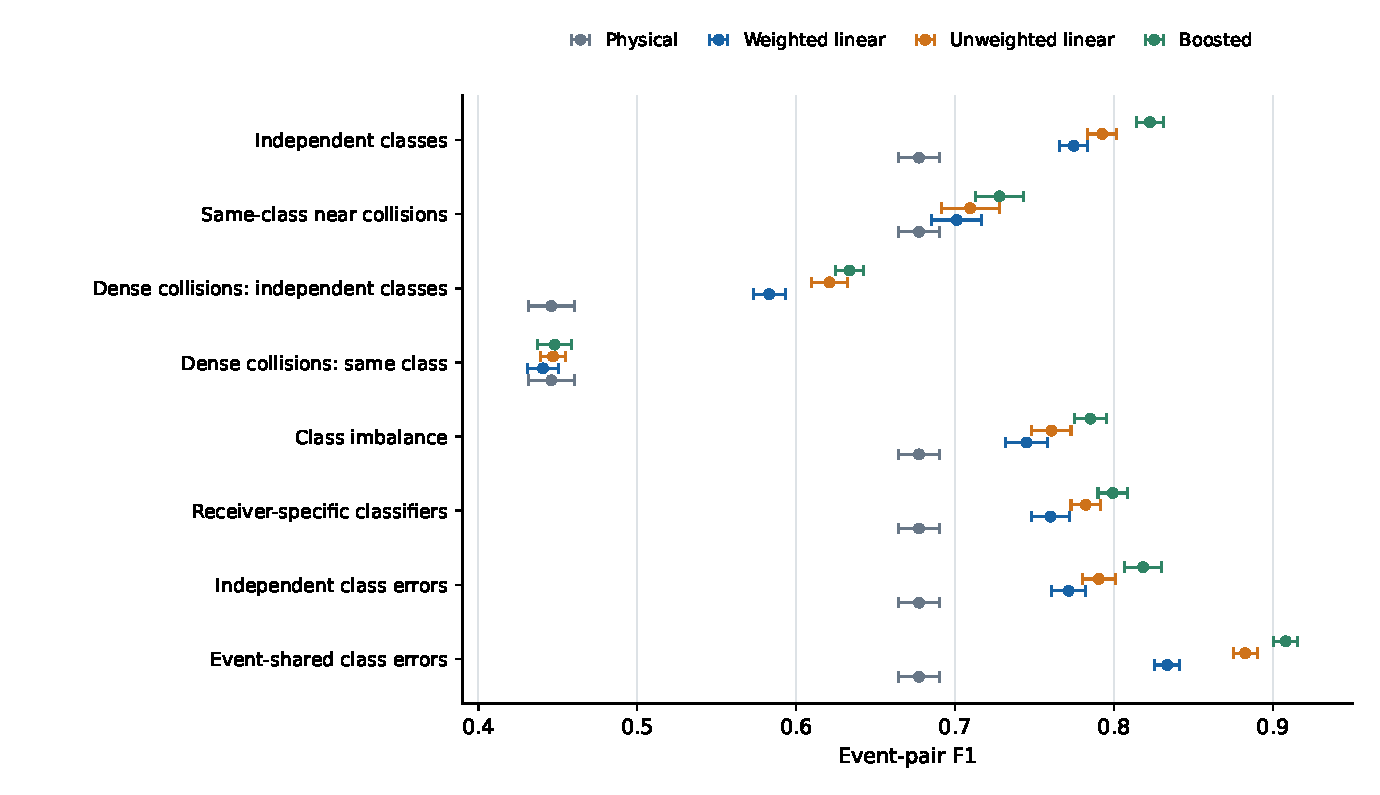
\includegraphics[width=\linewidth]{figures/deep_semantic_stress.pdf}
\caption{Semantic interventions on independent descriptor scenes. All class maps are supplied. Error bars use replication-level intervals. The dense same-class condition shows no clear semantic advantage in this experiment. Shared within-event errors preserve compatibility despite wrong class predictions.}\label{fig:deep_semantic}
\end{figure}

Every semantic-only intervention preserves the physical report arrays. Physical-only F1 is consequently identical across those paired conditions. The dense pair has its own physical reference. Verification reproduces 800 nominal and dense source scenes exactly. Independent checks also compare 576 physical fields with the original generator across 48 condition--seed cases. Replacing event and clutter labels leaves inference batches and checked predictions unchanged. All 12,800 outputs meet the receiver and gate constraints. The saved files include per-scene TP, FP, FN, all partition metrics, replication means, paired differences, and predictions. Pooled micro F1 is stored separately from scene-macro F1.
\FloatBarrier

\subsection{Public timestamp tails and a metadata clock comparator}
The script is \texttt{code/deep\_loed\_audit.py}. It reads the unchanged publisher sample and retained observation IDs. A tail diagnostic uses an absolute corrected time difference above 10 ms. It changes no inclusion decision or reference label. Table~\ref{tab:deep_loed_tail} shows all six captures, including April's lack of a cross-gateway reference pair.

\begin{table}[!htb]\caption{Corrected reference-pair time differences. Tail means an absolute difference above 10 ms. The last column counts tails with different reported channels. The 2019 receiver pair has no supported clock correction. Every central 2020 pair has matching channels. All records remain in the evaluation.}\label{tab:deep_loed_tail}
\scriptsize\setlength{\tabcolsep}{3pt}\begin{tabularx}{\linewidth}{@{}Yrrrrr@{}}\toprule
Capture & Reference pairs & Median ($\mu$s) & $Q_{0.99}$ (ms) & $>10$ ms & Channel mismatch in tail \\\midrule
2019-03-03 & 1 & 66771.6 & 66.772 & 1 & 0 \\
2019-04-02 & 0 & -- & -- & -- & -- \\
2020-05-02 & 256 & 4.0 & 2100.826 & 5 & 5 \\
2020-07-03 & 434 & 5.0 & 3.025 & 4 & 4 \\
2020-08-03 & 903 & 16.0 & 0.146 & 0 & 0 \\
2020-09-02 & 514 & 15.0 & 2.122 & 2 & 2 \\
\bottomrule\end{tabularx}
\end{table}

The eleven 2020 tail pairs have matching full PHY payloads, device addresses, frame counters, and spreading factors, but different channel frequencies. Each complete payload occurs in exactly two raw rows at two gateways, both with valid CRC, so they pass the existing one-record-per-gateway rule and five-second raw-span exclusion. The raw sample contains only one time field and cannot distinguish repeated transmissions from metadata errors. This reference ambiguity remains unresolved.

July's 434 sorted residuals have median $5\,\mu$s and 95th percentile $22\,\mu$s. Its 0.99 quantile has zero-based rank 428.67. Linear interpolation uses 2.120 and 3.471 ms. Its 0.999 quantile has rank 432.567 and uses 2.136977 and 4.201604 s. This gives 3.307620509 s. The endpoint record permits direct reproduction of the jump. Supported-pair raw signed medians from May through September are 0.999985, 0.999986, 1.000001, and 1.000000 s. These central shifts do not explain the seconds-long tails.

The alternative clock estimator receives only training day, gateway, timestamp, channel, and spreading factor. It forms matching-channel and matching-SF candidate lags in $[-5,5]$ s. Histogram bins are 1 ms wide. The strongest bin defines a refinement neighborhood of $\pm5$ ms. At least ten entries are required in the peak bin. At least twenty are required in the refinement. The peak must be at least five times the larger of one and the 99th percentile of all bin counts. It must also be at least twice the larger of one and the strongest bin beyond 10 ms from its center. Supported pair lags enter the same count-weighted least-squares clock system as the reference method. Unsupported corrections remain zero.

The 2020 pair supplies 343 metadata candidates. Its peak bin has 242 entries. The refinement has 251. The median lag is 0.999985 s. The 2019 pair supplies 38 candidates and peak count one. It remains unsupported. The largest difference between the two fitted receiver-correction vectors is $2.22\times10^{-16}$ s. Synthetic estimator checks recover a known 0.37 s shift with correct sign. Two equally strong separated modes are rejected. These checks do not represent new measured recordings.

\begin{table}[!htb]\caption{Clock fitting with unchanged public test reports. Reference support counts training payload matches. Metadata support counts lags in the fixed refinement neighborhood. Scorer fitting, gate calibration, and population selection remain reference-assisted. Both clock fits give identical test partitions.}\label{tab:deep_loed_clock}
\small\setlength{\tabcolsep}{3pt}\begin{tabularx}{\linewidth}{@{}Yrrrrr@{}}\toprule
Clock fit & Training support & Lag (s) & TP / FP / FN & $G$ (ms) & Packet F1 \\\midrule
Payload-reference median & 256 & 0.999985 & 1411 / 1 / 6 & 3.025 & 0.9975 \\
Metadata lag mode & 251 & 0.999985 & 1411 / 1 / 6 & 3.025 & 0.9975 \\
\bottomrule\end{tabularx}
\end{table}

The estimator settings are fixed for this secondary comparison without selection on test F1. Because the public captures had already been inspected, the comparison is not an independent prospective deployment test. The 2019-only training setting changes gateway coverage and positive support together with date, so its zero F1 cannot isolate temporal drift. All raw tail rows, quantile endpoints, support counts, fitted offsets, and test predictions are retained.
\FloatBarrier

\subsection{Fixed-registry report-path latency}
The script \texttt{code/deep\_runtime.py} uses ten fresh instances at each of $N=40,80,120$. The sizes use separate scenes. Their generator event counts are 18, 30, and 43. Selection uses report count alone. A random subset supplies the requested number of reports. The frozen weighted linear scorer is used throughout. Within each instance, every decoder receives the same reports and score model.

The timed path starts with native feature construction. It includes frozen scoring and event decoding. Descriptor generation, file I/O, waveform processing, and offline map fitting are excluded. Greedy and restart paths use the median of three contiguous measurements per instance. MILP uses one solve per instance. Initialization occurs outside the intervals. Reference metrics and feasibility checks also occur outside the intervals. The full triangle MILP includes sparse construction and label reconstruction in its reported path time. Preallocated sparse arrays reduce Python object overhead. The mathematical formulation is unchanged.

\begin{table}[!htb]\caption{Fresh fixed-registry report-path measurements. Each size uses ten independently seeded scenes. Median and maximum refer to instance-level path times. F1 averages ten scene values. The one-second cap applies to the solver only. Model construction is included in the reported path. Every MILP result is proven optimal.}\label{tab:deep_runtime}
\small\setlength{\tabcolsep}{3pt}\begin{tabularx}{\linewidth}{@{}rYrrrrr@{}}\toprule
$N$ & Decoder & Median (ms) & Maximum (ms) & Event F1 & Proven / 10 & Timeouts \\\midrule
40 & Greedy & 0.64 & 0.69 & 0.8068 & -- & -- \\
40 & Restart & 2.52 & 2.69 & 0.7841 & -- & -- \\
40 & MILP & 34.56 & 37.53 & 0.7781 & 10 & 0 \\
80 & Greedy & 1.80 & 1.92 & 0.7673 & -- & -- \\
80 & Restart & 8.03 & 8.50 & 0.7653 & -- & -- \\
80 & MILP & 284.37 & 335.45 & 0.7705 & 10 & 0 \\
120 & Greedy & 3.63 & 3.85 & 0.7830 & -- & -- \\
120 & Restart & 17.73 & 18.10 & 0.7841 & -- & -- \\
120 & MILP & 956.65 & 1014.16 & 0.7836 & 10 & 0 \\
\bottomrule\end{tabularx}
\end{table}

All 30 solves prove optimality without reaching the requested solver limit. The largest 120-report path takes 1014.16 ms because construction precedes optimization. These times describe the tested full formulation and environment, rather than a bound on all MILP implementations. At 40 reports, greedy mean event F1 is 0.8068 and MILP F1 is 0.7781. More objective search need not improve event accuracy. Different scenes and event densities also prevent a size-only interpretation of F1 changes across rows.

One separate Windows process measures a 120-report solve's memory. Its resident working set is 146,747,392 bytes before the solve. Peak working set reaches 650,665,984 bytes, or about 620.5 MiB. This includes Python, numerical libraries, sparse construction, and HiGHS. Initial sparse arrays occupy 40,440,960 bytes. The process peak is a measured example, not a memory upper bound. The case has 7140 variables and 842,520 triangle inequalities.

\subsection{Files and commands for the independent validation}
All new scientific outputs are under \texttt{results/deep\_revision/}. Mapping outputs are in \texttt{mapping}. Semantic interventions are in \texttt{semantic\_stress}. The remaining folders are \texttt{loed}, \texttt{runtime}, and \texttt{models}. Each experiment records its protocol, seeds or input identifiers, parameters, and checks. The dependency lock remains \texttt{requirements-review-lock.txt}. The following commands run from this project folder:
\begin{verbatim}
python code/deep_revision.py --task all
python code/deep_revision.py --task verify
\end{verbatim}
The first command executes the added experiments sequentially. The second checks retained outputs and invariants. Old scientific results remain in their original subdirectories. All comparisons use scene- or replication-level summaries as stated. Repeated solver or scorer evaluations do not create additional independent scenes.
